\chapter{Background}

\section{Port scanning}

Among the various techniques used for port scanning, the most common one is scanning for open TCP ports. TCP (Transmission Control Protocol) is a connection-oriented protocol utilized for reliable data transmission between two devices, requiring two sockets representing the endpoints of the connection. During the establishment of a TCP connection, a three-way handshake is performed, in which SYN (synchronize) and ACK (acknowledge) packets are exchanged between the two devices to establish the connection~\citescientific{de1999}.
Port scanners take advantage of the three-way handshake to identify open ports on a target system. The scanner sends a SYN packet to the target system and waits for a response. If the port is open, the target system responds with a SYN-ACK (synchronize-acknowledge) packet. The scanner then responds with an ACK packet to establish the connection. If the port is closed, the target system responds with a RST (reset) packet. This process is depicted in Figure~\ref{fig:open-vs-closed}.

\begin{figure}[h]
    \centering
    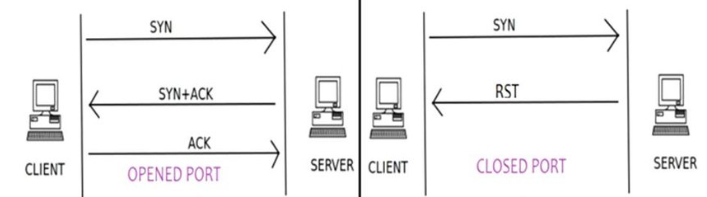
\includegraphics[width=15cm, height=15cm, keepaspectratio]{background/img/open_vs_closed_port.png}
    \caption{Open vs. closed port TCP connection~\protect\citescientific{Elijla2013}}
    \label{fig:open-vs-closed}
\end{figure}

Although other TCP header flags, such as FIN (finish), URG (urgent), and PSH (push), can also be utilized by port scanners to identify open ports, SYN scan is the most commonly used technique. This is because it is faster and less likely to be detected by intrusion detection systems (IDS) than other methods. 

\section{Browser-based vs. Regular Port scanning}

As this paper is focused on browser-based port scanning, it is important to explain why we make the distinction between regular port scanning and browser-based port scanning. 
There are two major differences, being the type of port scan attacks that we can do, as well as the difference in attack methodology that we employ. 
Regular port scanning is a lot more common, and there are many different types of attacks. 
The main distinction is that regular port scanning can perform protocol level scans. 
These type of scans can be very powerful, as small implementation differences at the OS level can be enough to establish a unique fingerprint of a system. 

In contrast, the scope of browser-based port scanning is defined by the functionality accessible through the abstraction layers of the JavaScript APIs, imposing limitations on its capabilities.
For instance, client-side JavaScript code using the WebSocket protocol cannot create UDP connections, and plain TCP connections cannot be opened either. In order to perform browser-based port scanning, we have to use the abstraction layers that are built on top of the TCP protocol, and leverage JavaScript APIs to send network requests. Figure~\ref{fig:js-network-stack} illustrates this, with the top (blue) layer representing the JavaScript APIs.

\begin{figure}[h]
    \centering
    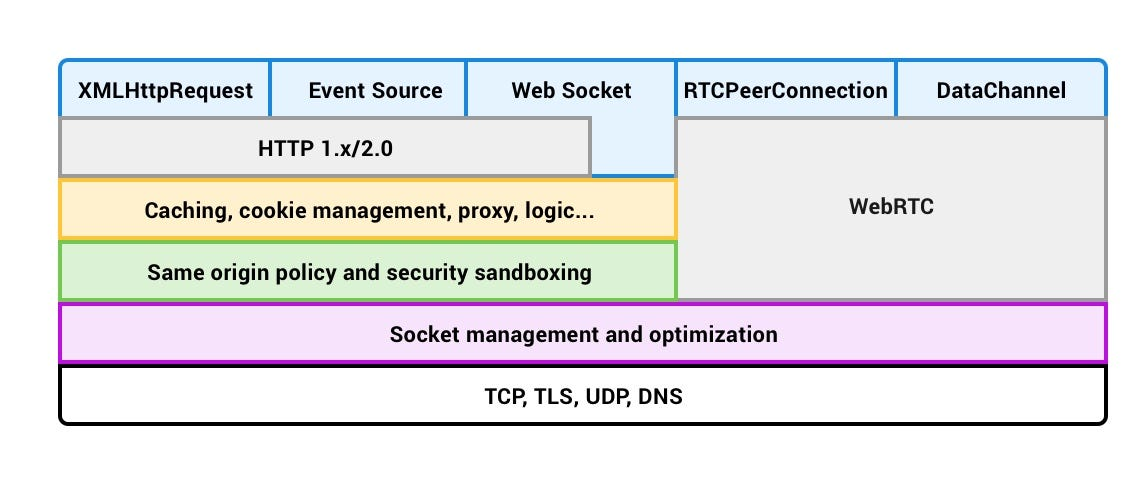
\includegraphics[width=15cm, height=15cm, keepaspectratio]{background/img/js_network_stack.jpg}
    \caption{JavaScript network layer~\protect\citearticle{medium_js_networking}}
    \label{fig:js-network-stack}
\end{figure}

This is the main technical difference between regular port scanning and browser-based port scanning, browser-based port scanning operates at layer 7 in the OSI model~\citescientific{kumar2014}, while regular port scanning can also operate at lower levels in the OSI model, such as layer 4. 
This makes regular port scanning much more powerful.
Additionally, the browser sandbox has several security measures that will make port scans less successful, most importantly, the Same-Origin policy~\citetechnical{w3c_same_origin_policy, same_origin_mozilla} restricts how a script can interact with a resource from another origin. Cross-Origin Resource Sharing (CORS)~\citetechnical{cors,fetchspec} headers can be configured to grant access to cross-domain resources. 
Aside from the technical scanning capabilities, the attack methodology is different, and this is what makes browser-based port scanning an interesting topic for research. 
Unlike regular port scanning, which embodies an active stance, browser-based port scanning adopts a passive stance. 
A website can discretely target its visitors without actively probing IPs or initiating network requests. The onus of initiating the attack rests on the user's act of visiting the website. 
While a website could initiate a regular port scan to the user's IP address, this type of attack would be much more intrusive and likely blocked by a firewall or router.

The crucial difference between browser-based port scanning and regular port scanning is that a browser-based port scan is executed locally on the user's machine, as opposed to originating from a server. 
This makes the attack a lot less intrusive, and not as easily detectable by intrusion detection systems. 
Not only is the attack not as easily detected, more importantly, the attack is not as easily prevented.
As the JavaScript is running locally on the user's system, there is likely nothing preventing the JavaScript from accessing the local network, besides the browser's sandbox environment.
The main area of research for browser-based port scanning is the fingerprinting capabilities. 
Browser-based port scanning is limited compared to regular port scanning, and security vulnerabilities are therefore unlikely, as it necessitates a breach of the browser's sandbox environment. 
For this reason, this paper focuses on privacy vulnerabilities, as ports can reveal a lot of information about the underlying system, and therefore enhance the capabilities of establishing a unique fingerprint.


\section{Ethics and Legality}
Port scanning is a technique that has raised ethical and legal concerns in the past~\citescientific{jamieson2001}. While some consider it a malicious activity, professionals often use it to identify network problems and detect vulnerabilities in their own network. In the majority of cases, port scanning does not harm the target system, and courts have typically ruled in favor of \\ it~\citescientific{Lyon2009}.
Recently, the Brandenburg Commissioner for Data Protection (DPA) examined the legality of port scans under GDPR regulations~\citeregulatory{gdpr}. In this particular case, port scans were used as a safeguarding mechanism to detect remote access tools such as AnyDesk, Remote Desktop Protocol, and TeamViewer. The DPA ruled in favor of port scanning, deeming it reasonable and understandable with no data protection concerns. This ruling establishes a precedent suggesting that port scanning is permissible under certain circumstances, even though enumerating the entire port range may not be lawful under GDPR~\citeregulatory{edpb_decision}.

While cookie consent is commonplace due to GDPR regulations, consenting to a local network search is not. Privacy experts criticized eBay when it was discovered that they had used port scans on the local network of their website visitors. This raises concerns about the lack of consent and transparency surrounding the use of port scanning in such circumstances~\citearticle{ebay_port_scans,forbes_ebay}.
Overall, while port scanning remains a controversial issue, the ruling by the Brandenburg DPA suggests that it can be lawful under certain circumstances. However, it is essential to ensure that individuals are aware of and understand the implications of such scans, particularly when performed without their consent.